\nte{Oct 07 2024 Mon (13:01:52)}{Consequences of Completeness}

\section{Nested Interval Property}
\label{sec:nested_interval_property}

\begin{theorem}[Nested Interval Property]
  For each $n \in \N$, assume we are given a closed interval $I_n = [a_n, b_n] =
  \left\{x \in \R \mid a_n \le x \le b_n\right\}$. Assume also that each $I_n$
  contains the next interval, i.e., $I_n \supseteq I_{n+1}$. Then, the
  resulting sequence of closed intervals
  \[%
    I_1 \supseteq I_2 \supseteq I_3 \supseteq \cdots
  ,\]%
  has a nonempty intersection. That is,
  \[%
    \bigcap_{n=1}^{\infty} I_n \neq \emptyset
  .\]%
\end{theorem}

\begin{proof}
  Define $A = \left\{a_n \mid n \in \N\right\}$. Because the intervals are
  nested, we see that every $b_n$ serves as an upper bound for $A$. Thus, we let
  $x = \sup(A)$. Now, consider a particular $I_n = [a_n, b_n]$. Because $x$ is
  an upper bound for $A$, we have $a_n \le x$. Since $x$ is the least upper
  bound, we have $x \le b_n$. This implies that $a_n \le x \le b_n$, which means
  $x \in I_n$, for every choice of $n \in \N$. Therefore, $x \in
  \bigcap_{n=1}^{\infty} I_n$.
\end{proof}

The Nested Interval Property can be viewed graphically, as shown below.
\begin{figure}[H]
  \centering

  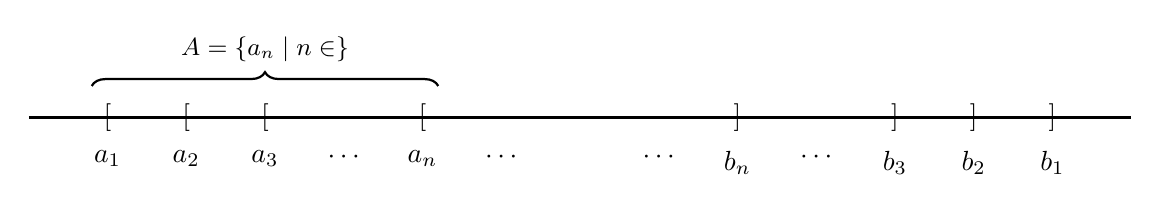
\begin{tikzpicture}
    \draw[thick] (-7, 0) -- (7, 0);

    \foreach \i/\pos in {1/-6, 2/-5, 3/-4, n/-2} {
      \node at (\pos, 0) {$[$};
      \node[below] at (\pos, -0.3) {$a_{\i}$};
    }
    \node[below] at (-3, -0.3) {$\cdots$};

    \foreach \i/\pos in {n/2, 3/4, 2/5, 1/6} {
      \node at (\pos, 0) {$]$};
      \node[below] at (\pos, -0.3) {$b_{\i}$};
    }
    \node[below] at (3, -0.3) {$\cdots$};

    \node[below] at (1, -0.3) {$\cdots$};
    \node[below] at (-1, -0.3) {$\cdots$};

    \draw[decorate,decoration={brace,amplitude=5pt},thick] (-6.2, 0.4) -- (-1.8, 0.4) node[midway, above=5pt] {{\small$A = \{a_n \mid n \in \N\}$}};
  \end{tikzpicture}
\end{figure}

\begin{example}
  The interval $I_n = \left[0, \frac{1}{n}\right]$, which is clearly $I_n
  \supset I_{n+1}$, since $\bigcap_{n=1}^{\infty} = \{0\}$.

  The counter example is $I_n = \left(0, \frac{1}{n}\right)$ because
  $\bigcap_{n=0}^{\infty} I_n = \emptyset$.
\end{example}

\begin{proof}
  Let $A = \left\{a_n \mid n \in \N\right\}$. From this, we know that $a_n \le
  b_n$ and $I_n \supseteq I_{n+1}$. From this, we know that $a_n \le b_1$,
  $\forall n \in \N$. This means that $A$ is bounded.

  By the Axiom of Completeness, $A$ has a least upper bound, $s = \sup(A)$.
  Then, $a_n \le s$, $\forall a_n \in A$. Since $s$ is the least upper bound, we
  get $s \le b_n$, giving us
  \[%
    a_n \le s \le b_n, \forall n \in \N \iff s \in \bigcup_{n=0}^{\infty} I_n
  .\qedhere\]%
\end{proof}

\begin{proposition}
  The set $\N$ is unbounded.
\end{proposition}

\begin{proof}
  Assume, for contradiction, that $\N$ is bounded above. Then, it follows that
  we can set $\alpha = \sup(\N)$. If we consider $\alpha - 1$, then we no longer
  have an upper bound for $\N$, and therefore, there exists an $n \in \N$
  satisfying $\alpha - 1 < n$, which is equivalent to $\alpha < n + 1$. Since we
  have $n + 1 \in \N$, this contradicts the assumption that $\alpha$ is the
  least upper bound of $\N$.
\end{proof}

\begin{theorem}[Archimedian Property] $ $
  \begin{enumerate}
    \item Given any number $x \in \R$, $\exists n \in \N$ satisfying $n > x$.

    \item Given any real number $y > 0$, $\exists n \in \N$ such that
      $\sfrac{1}{n} < 1$.
  \end{enumerate}
\end{theorem}

\begin{proof} $ $
  \begin{enumerate}
    \item Property (i) follows given that $\N$ is unbounded.

    \item Apply property (i) with $x = \sfrac{1}{y} > 0$. \qedhere
  \end{enumerate}
\end{proof}

% section nested_interval_property (end)

\section{Density of $\Q$ in $\R$}
\label{sec:density_of_q_in_r_}

\begin{theorem}[Density of $\Q$ in $\R$]
  Between any two real numbers $a$ and $b$ with $a < b$, there exists a rational
  number $q$ such that $a < q < b$.
\end{theorem}

\begin{proof}
  Let $a > 0$, giving us $0 < a < b$. Then, $b - a > 0$. By the archimedean
  property, $\exists n \in \N$ such that $\sfrac{1}{n} < b - a \iff a < b -
  \sfrac{1}{n}$.

  There is an $m \in \N$ such that $m - 1 \le na \le m \iff \frac{m - 1}{n} \le
  a \le \frac{m}{n}$.

  On the right hand side, we have $a \le \sfrac{m}{n}$, and on the left hand
  side, we have
  \begin{align*}
    \phantom{\implies}\quad&m \le an + 1 \\
    \implies\quad&\frac{m}{n} \le b \\
    \iff\quad&a \le \frac{m}{n} \le b
  .\qedhere\end{align*}
\end{proof}

Essentially, there are an infinite number of rational numbers between any two
real numbers, giving us
\[%
  a < r_1 < r_2 < r_3 < \dots < b
.\]%

\begin{corollary}
  Between any two real numbers $a < b$, then there are infinitely many
  irrational numbers.
\end{corollary}

\begin{proof}
  Assume $a > 0$. Given $a < b$, then $a - \sqrt{2} < b - \sqrt{2}$. By the
  density of $\Q$, then $\exists r \in \Q$ such that $a - \sqrt{2} < r_1 < b -
  \sqrt{2} \implies a < r + \sqrt{2} < b$. Since $r$ is rational, then $r +
  \sqrt{2}$ is irrational.
\end{proof}

% section density_of_q_in_r_ (end)

\section{Square Roots}
\label{sec:square_roots}

\begin{proposition}
  There exists a real number $\alpha$ satisfying $\alpha^2 = 2$.
\end{proposition}

\begin{proof}
  Let $S = \left\{x \in \R \mid x^2 < 2\right\}$. Then $S$ is bounded, nonempty,
  and has a least upper bound. Let $\alpha = \sup(S)$. We want to show $\alpha^2
  = 2$ by showing that $\alpha^2 \nless 2$ and $\alpha^2 \ngtr 2$.

  \textbf{Case 1} ($\alpha^2 \nless 2$): Suppose $\alpha^2 < 2$. We consider
  \begin{align*}
    \left(\alpha + \frac{1}{n}\right)^2 &= \alpha^2 + \frac{2\alpha}{n} + \frac{1}{n^2} \\
                                        &< \alpha^2 + \frac{2\alpha + 1}{n}
  .\end{align*}
  Since $\alpha^2 < 2$, we can choose $n$ large enough such that
  \[%
    \alpha^2 + \frac{2\alpha + 1}{n} < 2 \iff 0 < \frac{2\alpha + 1}{2 - \alpha^2} < n
  .\]%
  By the archimedian property, there is an $n \in \N$ such that
  \[%
    \left(\alpha + \frac{1}{n}\right)^2 < 2 \implies \alpha + \frac{1}{n} \in S
  ,\]%
  but $\alpha$ is the least upper bound, which is a contradiction. Therefore,
  $\alpha \nless 2$.

  \textbf{Case 2} ($\alpha^2 \ngtr 2$): Suppose $\alpha^2 > 2$. We consider
  \begin{align*}
    \left(\alpha - \frac{1}{n}\right)^2 &= \alpha^2 - \frac{2\alpha}{n} + \frac{1}{n^2} \\
                                        &> \alpha^2 - \frac{2\alpha}{n}
  .\end{align*}
  Since $\alpha^2 > 2$, we can choose $n$ large enough such that
  \[%
    \alpha^2 - \frac{2\alpha}{n} > 2 \iff 0 < \frac{2\alpha}{\alpha^2 - 2} < n
  .\]%
  By the archimedian property, there is an $n \in \N$ such that
  \[%
    \left(\alpha - \frac{1}{n}\right)^2 > 2 \implies \alpha - \frac{1}{n} \notin S
  ,\]%
  but $\alpha$ is the least upper bound, which is a contradiction. Therefore,
  $\alpha \ngtr 2$.
\end{proof}

% section square_roots (end)

\newpage
